% --------------------------------------------------------------------------
% Template for DCASE 2017 paper; to be used with:
%          dcase2017.sty  - DCASE 2017 LaTeX style file, and
%          IEEEbib.bst - IEEE bibliography style file.
% Adapted from spconf.sty and waspaa15.sty
% --------------------------------------------------------------------------

\documentclass{article}
\usepackage{dcase2017,amsmath,graphicx,url,times,booktabs,tabularx}

\usepackage{setspace}
\usepackage{enumitem}
\usepackage{csquotes}
\usepackage{xcolor}
\usepackage{tcolorbox}
\usepackage{placeins}
\usepackage{booktabs}
\usepackage{multirow}
\usepackage{array}
\usepackage{caption}
\usepackage[hidelinks,bookmarks=false,draft]{hyperref}

% --------------------
\def\defeqn{\stackrel{\triangle}{=}}
\newcommand{\symvec}[1]{{\mbox{\boldmath $#1$}}}
\newcommand{\symmat}[1]{{\mbox{\boldmath $#1$}}}

\makeatletter
\def\bstctlcite{\@ifnextchar[{\@bstctlcite}{\@bstctlcite[@auxout]}}
\def\@bstctlcite[#1]#2{\@bsphack
  \@for\@citeb:=#2\do{%
    \edef\@citeb{\expandafter\@firstofone\@citeb}%
    \if@filesw\immediate\write\csname #1\endcsname{\string\citation{\@citeb}}\fi}%
  \@esphack}
\makeatother

% --------------------
\title{The details that matter: Frequency resolution\\of spectrograms in acoustic scene classification}


% --------------------
\name{Karol J. Piczak\thanks{\hspace{-1.6em}The source code for this study can be found at:\newline \hspace*{0.1em} \href{https://github.com/karoldvl/paper-2017-DCASE}{https://github.com/karoldvl/paper-2017-DCASE} }}
\address{Institute of Computer Science\\
Warsaw University of Technology}

\begin{document}

\bstctlcite{IEEEexample:BSTcontrol}

\ninept
\maketitle

\begin{sloppy}


% --------------------
\begin{abstract}
This study describes a convolutional neural network model submitted to the acoustic scene classification task of the DCASE 2017 challenge. The performance of this model is evaluated with different frequency resolutions of the input spectrogram showing that a higher number of mel bands improves accuracy with negligible impact on the learning time. Additionally, apart from the convolutional model focusing solely on the ambient characteristics of the audio scene, a proposed extension with pretrained event detectors shows potential for further exploration.
\end{abstract}

\begin{keywords}
acoustic scene classification, spectrogram, frequency resolution, convolutional neural network, DCASE~2017
\end{keywords}


% --------------------
\vspace{-4pt}
\section{Introduction}

The area of environmental sound classification has recently experienced a~significant increase in the quantity of performed studies. One of the main driving factors in 2016 was the organization of the first DCASE workshop~\cite{DCASE2016workshop}, complemented by an open challenge focusing on the detection and classification of acoustic scenes and events. This unique opportunity enabled researchers to exchange ideas and evaluate various approaches on a common set of tasks and datasets, a valuable initiative which continues in 2017 with a~second installment of the workshop~\cite{DCASE2017challenge}.

Looking at previous submissions to this challenge, a clear picture emerges on how diverse the methods employed to tackle these tasks can be. In 2013, when the very first DCASE challenge~\cite{stowell2015} was organized, although most approaches used a support vector machine (\textit{SVM}) classifier, the input frames spanned a vast range of features:

\begin{itemize}[noitemsep,topsep=0pt,leftmargin=12pt,partopsep=4pt]
\itemsep0em

\item mel-frequency cepstral coefficients (\textit{MFCC})~\cite{geiger2013, nogueira2013, roma2013},
\item mel spectrograms processed through a sparse RBM extractor~\cite{nam2013},
\item statistics from a~cochleogram based on a tone-fit algorithm~\cite{krijnders2013},
\item responses of modulation tuned filters (2D Gabors)~\cite{patil2013},
\item visual features (\textit{HOG}) computed on a constant-Q transform~\cite{rakotomamonjy2015}.

\end{itemize}

\noindent At the same time, other teams evaluated the usefulness of hidden Markov models (\textit{HMM})~\cite{chum2013}, an i-vector approach combined with MFCCs~\cite{elizalde2013}, bagging of decision trees with MFCCs and wavelets~\cite{li2013} and a random forest classifier working on an embedding through dissimilarity representation~\cite{olivetti2013}.

In contrast, the DCASE 2016 challenge saw an emergence of deep learning techniques with numerous systems shifting to deep neural networks (\textit{DNN})~\cite{mun2016, takahashi2016, xu2016, choi2016}, convolutional neural networks~\cite{han2016, valenti2016, lidy2016, phan2016, battaglino2016, cakir2016}, recurrent models~\cite{vu2016, bae2016, zoehrer2016, hayashi2016, adavanne2016} and their fusions with other approaches like the i-vector~\cite{eghbal2016}. Although MFCCs were still widely encountered as input features in sound event detection, more low-level representations such as mel band energy and various forms of spectrograms were much more common in the acoustic scene classification task.

When developing models relying on spectrograms as their input, one of the decisions that has to be made is the resolution of the data generated in the preprocessing step. What should it be? One obvious response is: \enquote{the higher, the better}. As visualized by Figure~\ref{fig:spectrograms}, choosing a more fine-grained representation means less information is being lost at the very beginning and this should hopefully allow for more nuanced differentiation between similar training examples in later stages. However, there are three countervailing issues that we have to take into consideration here.

\begin{figure}[b]
  \vspace{-12pt}
  \centering
  \centerline{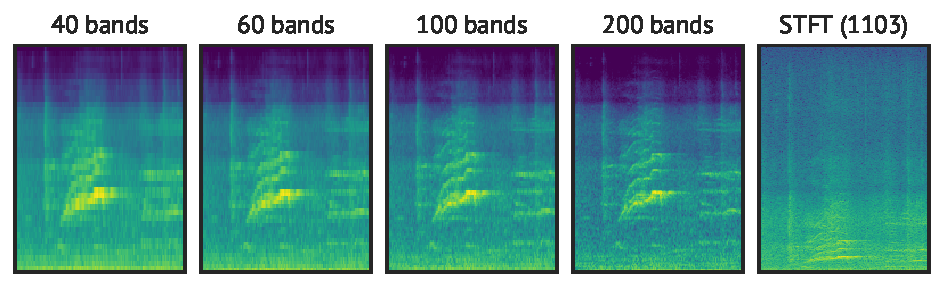
\includegraphics[width=\columnwidth]{figures/spectrograms.pdf}}
  \vspace{-6pt}
  \caption{A visual comparison of 3-second-long fragments of spectrograms with different frequency resolutions (first four use a mel scale, the last one is a plain STFT).}
  \label{fig:spectrograms}
  \vspace{-2pt}
\end{figure}

First of all, although increasing the time and frequency resolution of the employed representation may be desirable, the uncertainty principle imposes a theoretical limit on how these two can be combined. It is always a trade-off. Wide windows give good frequency resolution, but their temporal resolution is affected for the worse. Narrow windows behave in the opposite way.

One can counter this claim by stating that, theoretical limits notwithstanding, in most cases it is still possible to maintain a temporal resolution sufficient for an audio classification task while using wider windows. Even then, however, a practical aspect of resource constraints remains. Will the impact on memory and storage requirements introduced by a higher resolution be acceptable in a~given application? Is a longer computation time, both in the preprocessing and learning phase, really worth it? Especially in scenarios combining real-time processing with deployment on low-power devices these issues can become crucial.

Finally, dimensionality reduction of the input data is a proven way to facilitate learning. Looking from this perspective, a single audio frame of 10 milliseconds, sampled at 44.1 kHz, contains 441 datapoints in its raw form. On the contrary, MFCCs can succinctly describe it with only a~dozen of coefficients. With longer frames the discrepancy will be even more pronounced. Therefore, a valid concern arises whether a~high-resolution spectrogram with hundreds of frequency bands will not become an overkill that effectively impedes efficient learning.

Evaluating related works in this area, it seems indeed that the prevailing tendency is to limit the number of computed frequency bands to less than 100. Although greater values can be occasionally encountered (100 in~\cite{hayashi2016}, 128 in~\cite{salamon2017}, 150 in~\cite{giannoulis2016} and even 1025 in~\cite{zoehrer2016}), 60 bands~\cite{valenti2016,battaglino2016} and 40 bands~\cite{xu2016,bae2016,adavanne2016, sobieraj2016} are the dominant option. This would imply either that the gains potentially achievable from a higher resolution are counterbalanced by other negative factors, or that the issue is deemed, so far at least, only tangential to the actual problem of model construction and has not received much attention of itself.

This specific research question is the main motivation behind this study. A thorough analysis of all the issues voiced in the introduction is not possible in a scope of a short paper, so it will be limited to an evaluation of a single submission to the acoustic scene classification task of the DCASE 2017 challenge~\cite{DCASE2017challenge}. Nevertheless, it will hopefully signal whether this problem could be worth investigating further in a more generalized manner.

\vspace{-2pt}

% --------------------
\section{Experiment setup}

\subsection{Task and dataset}

The goal of the acoustic scene classification task proposed in the DCASE 2017 challenge is to determine the context of a given recording by choosing one appropriate label from a set of 15 predetermined acoustic scenes. For each scene, there are 312 audio segments in the development dataset with each segment having a length of 10 seconds and a sampling rate of 44.1 kHz. The challenge organizers prearranged the development dataset into 4 folds for comparable cross-validation in such a manner that segments originating from one physical location are contained in the same fold. The final scoring of submitted systems is based on the fraction of correctly classified segments from the evaluation dataset. Further information about the recording and annotation procedure can be found in the paper describing the dataset~\cite{mesaros2016}.

\vspace{-4pt}

\subsection{Data preprocessing}

The first step of the proposed solution consists in converting all the provided recordings into spectrograms with \textit{librosa v0.5.1}~\cite{librosa0.5.0}. Mel spectrograms are created with an FFT window length of 50~ms (2205 samples), hop length of 20~ms (882 samples), and a number of bands that is either 40, 60, 100 or 200, in all cases covering a~frequency range of up to 22050~Hz. Additionally, a plain STFT spectrogram (1103 bands) is created with the same window and hop length for comparison. Finally, the spectrograms are converted to a~decibel scale and standardized by subtracting the mean and dividing by the standard deviation computed on a random batch of 1000 examples. In this manner, the resulting dimension of a 10-second-long segment representation is $b$ rows and $500$ columns, where $b$ is the number of generated frequency bands.

During training, slight data augmentation is introduced by a~uniformly distributed offset of the start time of up to 1 second. Moreover, in each case a randomly sized tail of the generated example is replaced with a different segment belonging to the same class, creating some additional variety in the training batches.

\vspace{-4pt}

\subsection{Model architecture}

Most acoustic scenes can be conceptually described as an ensemble of two distinct elements. The ambience layer consists of a nondescript theme recurring in the background with little to no change (e.g. sound of a noisy street). Every now and then a more specific event of a short-lived nature occurs (e.g. a book page being flipped in a library). In many situations the background information alone is quite sufficient for establishing an actual context with little ambiguity. However, browsing through the provided dataset and trying to deduce how human perception copes with such a task, it seems that in some cases very subtle clues (as the aforementioned page flipping) are the key elements that drastically shift the expectations between similar contexts (e.g. \textit{home} and \textit{library}).

Based on this observation, a natural question is whether a machine learning model incorporating such an assumption would be advantageous. On the other hand, taking into consideration the high accuracy of the baseline solution and the results of Mafra~et~al.~\cite{mafra2016} where the authors indicate that good results can be obtained by representing each recording with only a single averaged frame, it is thus very likely that a good architecture should not be overly complicated in this case.

\begin{figure}[t]
  \centering
  \centerline{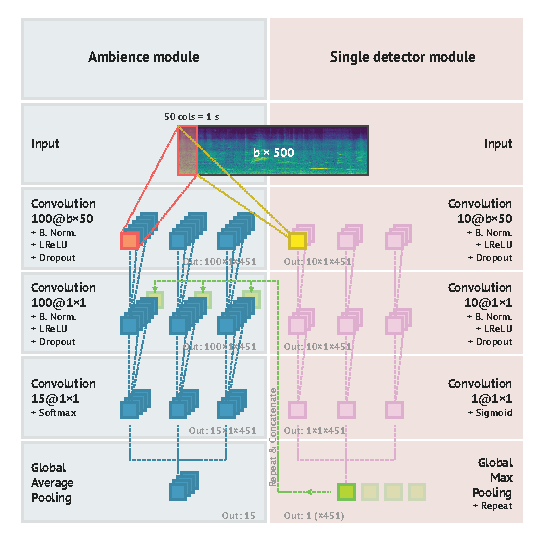
\includegraphics[trim={3mm, 3mm, 3mm, 3mm},clip,width=\columnwidth]{figures/model.pdf}}
  \caption{A schematic of the model with its ambience part and a~possible extension with a detector module.}
  \label{fig:model}
  \vspace{-8pt}
\end{figure}

Therefore, the system described in this work has a very simple design, coming in two flavors depicted in Figure~\ref{fig:model}. The first variant is a three block convolutional network focusing on processing the ambience content. Its first layer takes the whole input spectrogram ($b \times 500$) and applies a convolution with a stride of 1, filter size of $b \times 50$ (i.e.~over fragments of 1~second) and the number of filters set at 100. The response is batch normalized and processed through a~LeakyReLU activation ($\alpha = 0.3$) combined with dropout (\mbox{$p_\textrm{drop} = 0.25$}). The second processing block is identical, except for the filter size which in this case is reduced to $1 \times 1$, meaning that there is no spatial convolution but only aggregation across feature maps. The final layer consists of 15 convolutional filters of $1 \times 1$ and a softmax activation that is computed separately for each step. For training purposes, output probabilities are averaged with a global pooling layer. However, during the prediction step no pooling is performed, but instead these values are binarized with a threshold of $0.5$ and only then averaged over the whole time span, which is equivalent to a majority vote.

The second variant extends this model with a module that we will further call a \textit{detector}. An architecture of a detector is exactly the same as the already described ambience part with the difference that convolutional blocks use only 10 filters and the last layer consists of a single convolutional unit with sigmoid activation that is max-pooled over the whole time span. The rationale behind this is that the output of such a network should signal whether a given event (template match) has occurred anywhere in the whole recording. The whole variant then combines the ambient module with a~predefined number of detectors by concatenating their output to the input of the last convolutional layer (same global event detection value is repeated for each step of the ambient model).

Two remarks about the implications of such an architecture. First of all, while we are using a \enquote{convolutional} designation for this model, were it not for some subtle differences coming from the use of normalization layers and joint training, it could be validly understood as a simple multi-layer perceptron that is being applied to consecutive frames of the input, an approach very similar to the baseline implementation.

Moreover, by filling the first layer with filters of a very large size, spanning the whole frequency range, we can limit the impact of higher resolutions to this layer only. This means that the increase in computation time is not that severe. The prospects here would be much worse with networks stacking multiple layers of small-sized filters, where such changes propagate in the output dimensions of deeper layers, a drawback which should not be overlooked.

\begin{figure}[t]
  \centering
  \centerline{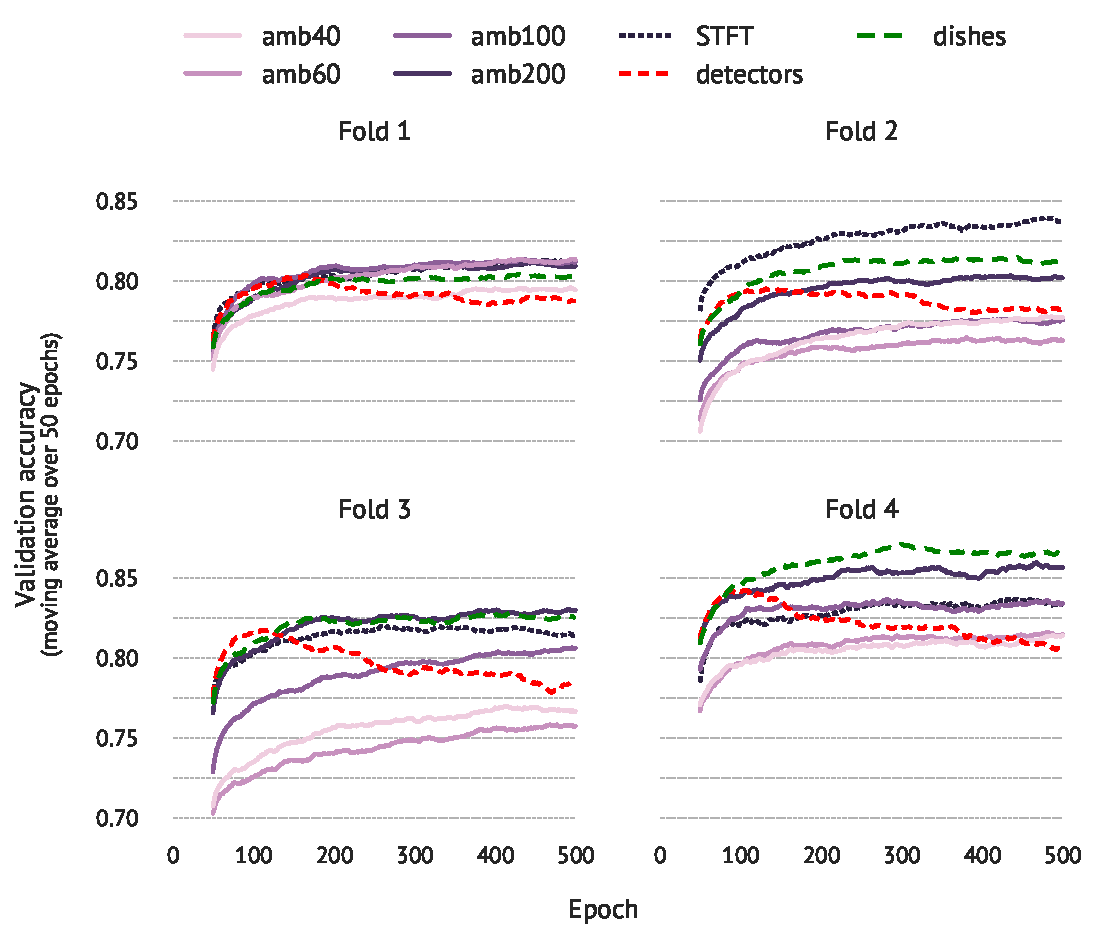
\includegraphics[width=\columnwidth]{figures/validation.pdf}}
  \vspace{-6pt}
  \caption{Comparison of validation accuracy for the evaluated systems achieved on the development dataset. Results are presented as a moving average over 50 epochs for better clarity.}
  \label{fig:validation}
  \vspace{-8pt}
\end{figure}

\vspace{-6pt}
\subsection{Training procedure}

Before training, all model weights are initialized with a \textit{He uniform}~\cite{he2015} procedure. Training is performed for 500 epochs with an \textit{Adam} optimizer (learning rate of $0.001$, batch size of 32) and a categorical cross-entropy loss function. 400 segments are carved out from the training fold as an additional holdout batch. The best performer on the holdout batch is retained as the final model, whereas validation results are calculated on a completely separate fold as provided by the organizers. Separate models are trained for each combination of training and validation folds. A hierarchical learning method similar to the one reported in~\cite{xu2016} was tentatively evaluated, however the difference achieved with the employed architecture was not noticeable enough to warrant further investigation.

\vspace{-6pt}

% --------------------
\section{Results}

\begin{figure}[t]
  \centering
  \centerline{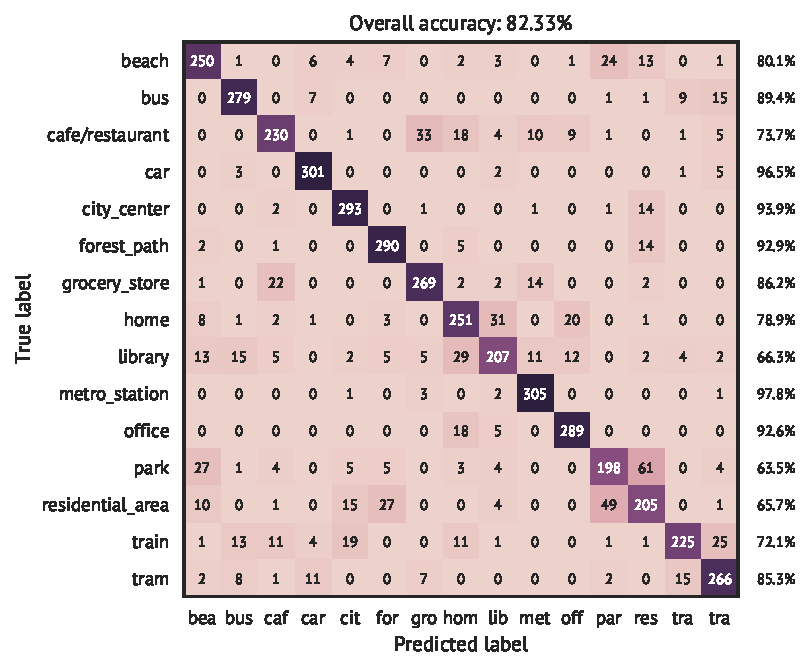
\includegraphics[width=\columnwidth]{figures/run_200_th_0_5.pdf}}
  \vspace{-6pt}
  \caption{Confusion matrix of the submitted \textit{amb200} model (ambience only, 200 mel bands) combined over all folds of the development set. The rightmost column presents class-wise accuracies.}
  \label{fig:confusion}
  \vspace{-8pt}
\end{figure}

\begin{figure}[b]
  \vspace{-6pt}
  \centering
  \centerline{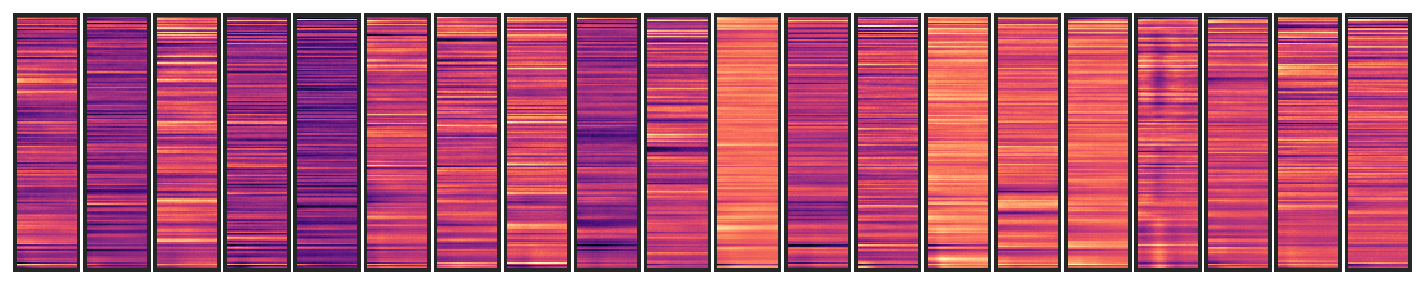
\includegraphics[width=\columnwidth]{figures/conv1_filters.pdf}}
  \caption{First 20 filters learned by the initial convolutional layer of the \textit{amb200} model (ambience only, 200 mel bands).}
  \label{fig:conv1_filters}
\end{figure}

The main system presented in this work, codenamed \textit{amb}, consisted solely of the ambience processing module (left part of Figure~\ref{fig:model}). Five variants of this model were evaluated, four using mel spectrograms with 40, 60, 100 and 200 frequency bands respectively and one working on STFT spectrograms with 1103 bands (denoted as \textit{STFT} later on). Additionally, a model combining the \textit{amb200} variant with 15 independent detector modules was created (\textit{detectors}). The results of these models are depicted in Figure~\ref{fig:validation} and presented in a numerical way in Table~\ref{tab:results}, while Figure~\ref{fig:confusion} more specifically details class-wise performance of the \textit{amb200} model.

The analysis of these results indicates that a higher number of mel frequency bands quite uniformly improves the achieved validation accuracy. There is almost a 4 percentage point difference between \textit{amb40} and \textit{amb200} variants, showing that, in this setup at least, higher resolution models have a greater predictive capacity. The \textit{STFT} variant is on average comparable to \textit{amb200}, it is however underperforming in fold~4 and strongly outperforming in fold~2. Taking into consideration the processing overhead (approximate epoch processing time on a GTX~980~Ti card was 23~s for \textit{amb40} up to 25~s for \textit{amb200} and 52~s for \textit{STFT}) the \textit{amb200} variant is a clear winner.

On the other hand, a disappointing behavior of the \textit{detectors} model combines poor validation accuracy with very high training time. It is quite evident that for this particular dataset the capacity of such an architecture is too high and after 100 epochs of training significant overfitting occurs. Therefore, an additional model \textit{dishes} is proposed. What is peculiar about it, it extends the \textit{amb200} model with only a single detector. Moreover, this detector module is separately pretrained on additional hand-annotations specifically created for this purpose indicating the occurrence of specific events in the \textit{cafe/restaurant} scene that could be described as sounds involving cups, plates, kitchenware etc. Unfortunately, due to time constraints and the effort involved in creating a more complete annotation of the dataset, it was not possible to evaluate a model with a broader range of pretrained detectors. However, taking into consideration that initial results reported here hint at a possible improvement, it could be an interesting further avenue for research. 

Finally, trying to understand a bit better on what is going on behind the scenes, we can see that the ambience model learns to be a strong frequency discriminator as seen both by the convolutional filters visualized in Figure~\ref{fig:conv1_filters} and examples of patterns that induce the strongest activation for a specific class (Figure~\ref{fig:max_activations}). This would explain why a high frequency resolution of the input data might be so important for this task. However, especially looking at Figure~\ref{fig:max_activations}, the perceptual differences are minuscule apart from some intricate patterns of narrow frequency bands, so a real question is on what is being learned. Is it actually the semantic differentiator between different types of scenes? In some cases, like interiors of vehicles, most probably yes. However, for classes such as \textit{home} or \textit{library} it is quite possible that these specific frequency patterns concentrate on what would be perceived by a human listener as recording artifacts. Further study would be required, but there is a high risk that the resulting model would be prone to adversarial attacks.

\begin{figure}[t]
  \centering
  \centerline{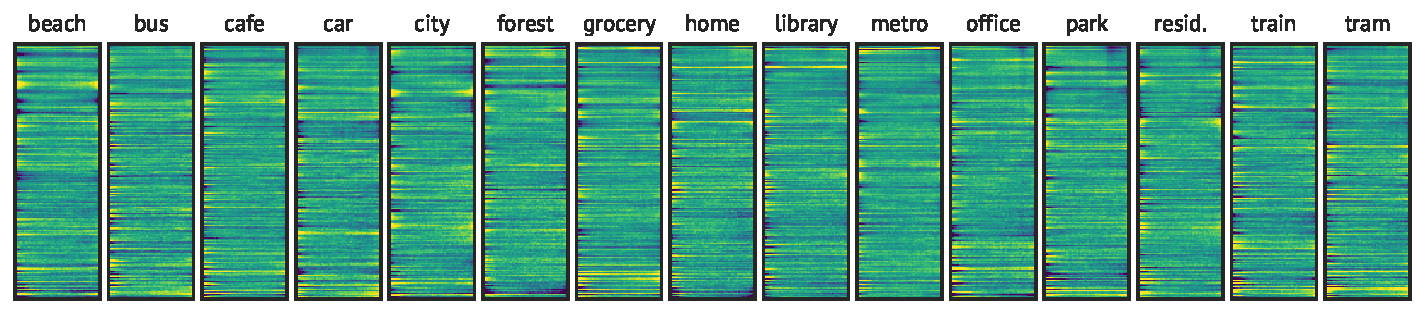
\includegraphics[width=\columnwidth]{figures/max_activations.pdf}}
  \caption{Synthetic examples of input patterns resulting in maximum output activation for a given class ($p_\textrm{class}(\symmat{X}) = 1.0$). Slight contrast squashing was applied for presentation purposes.}
  \label{fig:max_activations}
  \vspace{-6pt}
\end{figure}

\begin{table}[b]
	\renewcommand{\arraystretch}{1.2}
    \scriptsize
	\centering
    \caption{Results of the proposed systems.}
    \label{tab:results}
     \vspace{-2pt}
    \setlength{\tabcolsep}{0.8em}
	\begin{tabular}{l r r r r r r}
    \toprule
    \multicolumn{1}{l}{\multirow{2}[3]{*}{System}} & \multicolumn{5}{c}{Development} & \multicolumn{1}{c}{\multirow{2}[3]{*}{Final}} \\
    \cmidrule{2-6}
    & \multicolumn{1}{c}{Fold 1} & \multicolumn{1}{c}{Fold 2} & \multicolumn{1}{c}{Fold 3} & \multicolumn{1}{c}{Fold 4} & \multicolumn{1}{c}{1---4} & \\
    \cmidrule{1-1} \cmidrule{2-6} \cmidrule{7-7}
    amb40 & 79.4 (0.5) & 77.7 (0.8) & 76.7 (1.0) & 81.4 (1.0) & 78.8 & --- \\
    amb60 & 81.3 (0.6) & 76.3 (1.0) & 75.8 (0.9) & 81.5 (1.0) & 78.7 & 62.0 \\
    amb100 & 81.1 (0.6) & 77.5 (0.9) & 80.6 (0.7) & 83.4 (1.3) & 80.7 & 67.7 \\
    amb200 & 80.9 (0.8) & 80.2 (0.8) & 83.0 (0.9) & 85.6 (1.3) & 82.4 & 70.6 \\
    STFT & 81.1 (0.9) & 83.6 (0.8) & 81.4 (0.9) & 83.4 (1.3) & 82.4 & --- \\
    detectors & 78.7 (0.9) & 78.1 (1.1) & 78.6 (1.3) & 80.8 (1.4) & 79.1 & --- \\
    dishes & 80.3 (0.9) & 81.4 (0.7) & 82.6 (0.6) & 86.6 (1.0) & 82.7 & 69.6 \\
    \bottomrule
	\end{tabular}
    \vspace{6pt}
    \caption*{\footnotesize Mean (standard deviation) of validation accuracies across 50 final epochs of training on the development set and official evaluation results for submitted models. Values in percentages.}
    \vspace{-6pt}
\end{table}

% --------------------
\section{Conclusion}

This paper described a submission to the acoustic scene classification task of the DCASE 2017 challenge based on a convolutional neural network model specifically limited to focusing on the ambient characteristic of auditory scenes by average pooling responses for consecutive fragments of the recording. Experiments completed in this study showed that a very important determinant of the final performance in this task is the frequency resolution of the input representation being used, most probably due to the fact that the network is learning a form of a frequency discriminating function. Therefore, increasing the number of mel bands up to 200, well above what is most commonly encountered in related works, proved to be most effective. At the same time, using plain STFT spectrograms with even higher number of bands did not provide additional gains, while considerably increasing the computation time.

It is hard to tell in the scope of this work whether these results could be generalized for other contexts (e.g. event detection), where apart from the frequency content, changes in time also play a~crucial role. Concurrently, while the exact scope of the increase in the processing time when employing different types of models is not clear, a valid concern is whether the gains achieved will compensate for the longer training time, especially when using deep convolutional architectures with very small filters. This would have to be evaluated on a case-by-case basis. Nevertheless, the aim of this study is to underline that this hyperparameter should also be taken into consideration, even if only to squeeze some additional performance out of the very final model.

\vspace{-6pt}
% --------------------
\begin{spacing}{0.93}

\bibliographystyle{IEEEtran}
\bibliography{refs}

\end{spacing}

\end{sloppy}
\end{document}
